\documentclass{article}
\usepackage{amsmath}
\usepackage{amssymb}
\usepackage{graphicx}
\usepackage{gnuplottex}
\setcounter{page}{11}

\begin{document}
	\section{Ejercicio 2:}
		\subsection{Descripci\'on del problema:}
		El problema que se nos present\'o consist\'ia en, mediante un arreglo ya formado, crear uno nuevo que en la posici\'on $i$ de este nuevo arreglo tuviese la mediana del subarreglo ordenado que se forma del arreglo original entre las posiciones 0 a $i$.
		\\ La mediana para un arreglo de tama\~no \textit{n}  se calcula de la siguiente forma: si el arreglo tiene un tama\~no impar la mediana es \textit{x$_{(n+1)/2}$}; en cambio, si el tama\~no es par, es (\textit{x$_{(n)/2}$}+\textit{x$_{(n+1)/2}$})$/2$.
		\subsection{Resoluci\'on del problema:}
		Para resolver el problema se decidi\'o usar una estructura que consiste de cuatro observadores: dos heaps (un min heap y un max heap), un entero que contiene a la mediana y un entero que representa el tamaño del arreglo.
		\\ Para armar el arreglo que se va a devolver, se recorre el arreglo original, se toma el valor que est\'a en la posici\'on $i$ del arreglo original y luego se analiza el tama\~no del subarreglo (antes de agregar un nuevo n\'umero). En caso de que sea 0, quiere decir que esta vac\'io, entonces la mediana es el valor que tomamos.
		\\Si el subarreglo tiene un tama\~no impar, nos fijamos si el valor es mayor o menor que la mediana. En caso de que sea menor, se agrega el valor al max heap y la mediana al min heap, y si es mayor es al rev\'es. Luego, la mediana es la suma de las ra\'ices de los heaps dividido dos y se le suma 1 al tama\~no.
		\\En cambio, si el subarreglo tiene tama\~no par, tambi\'en nos fijamos si el valor es mayor o menor que la mediana. En caso de ser menor, se le agrega el valor al max heap y se desencola la ra\'iz del max heap y ese se transforma en la mediana, pero si es mayor se agrega el valor al min heap y se desencola la ra\'iz del min heap y ese se transforma en la mediana, y se le suma uno al tama\~no.
		\\Como dijimos, esto se va a hacer mientras se recorre el arreglo original, entonces cada vez que se agrega un nuevo valor a la estructura nos fijamos cual es la mediana y agregamos la mediana al arreglo que vamos a devolver.
		\subsection{Justificacion del algoritmo:}
		 La idea del algoritmo es que el tama\~no de los heaps siempre sea igual y de esa forma poder siempre ver f\'acilmente la parte que nos importa del subarreglo r\'apidamente y de una forma ordenada. Como ya se explic\'o anteriormente, antes de agregar un nuevo valor al subarreglo nos fijamos el tama\~no de este. Como caso base si el subarreglo tiene tama\~no 0 antes de agregar un n\'umero, cuando lo agreguemos va a tener tama\~no 1 y en ese caso ese mismo n\'umero va a ser la mediana, y los dos heaps tienen tama\~no cero.
		\\Ahora suponiendo que ambos heaps tienen el mismo tama\~no:
		\\ En caso de que antes de agregar un n\'umero el tama\~no sea impar, cuando lo agreguemos va a ser par, entonces por la f\'ormula para calcular la mediana tenemos que sumar los dos n\'umeros que est\'an en el medio y dividirlos por dos, pero antes de hacer eso hay que fijarse si el valor que se va a agregar es mayor o menor que la mediana y a qu\'e heap tendr\'ia que ir.
		\\Si el valor es menor que la mediana, se agrega el valor al max heap, que es donde est\'an los valores menores que la mediana, y la mediana se agrega al min heap, que es donde est\'an los valores mayores que la mediana, y de esta forma se mantiene el invariante de que los dos heaps tienen el mismo tamaño, y le mediana nueva se calcula con la f\'ormula previamente mencionada.
		\\ Si en cambio el tama\~no es par, cuando lo agreguemos va a ser impar, entonces la mediana va a ser el elemento que est\'a en el medio. Ahora nos fijamos si el valor a agregar es mayor o menor que la mediana, en caso de ser menor lo agregamos al max heap y desencolamos su ra\'iz, y esa va a ser la nueva mediana. En caso de ser mayor se agrega al min heap y luego se desencola la ra\'iz. La ra\'iz desencolada va a ser la nueva mediana, y los tama\~no de los heap se mantienen equivalentes.
		\subsection{Complejidad del algoritmo:}
		La complejidad de este algoritmo es de \textit{nlog(n / 2)}, que asint\'oticamente es equivalente a \textit{O(n)}, que es mejor que la cota que nos ped\'ian de \textit{n$^{2}$}, siendo \textit{n} la cantidad de n\'umeros que tiene el arreglo original. Esta complejidad se debe a que en cada iteraci\'on se realiza uno o dos adiciones a un heap, dependiendo esto del tama\~no del subarreglo, y se ven las ra\'ices de los heaps, pero al ser de tiempo constante esta funci\'on no suma a la complejidad, haciendo que cada adici\'on al subarreglo sea \textit{log(n)}. Como esto se realiza para todos los n\'umeros en el arreglo original, esto se realiza \textit{n} veces, haciendo que la complejidad total sea la dicha.
		\\Se sabe que los m\'etodos de des/encolar son de \textit{O(log n)} y ver la ra\'iz de \textit{O(1)} por la documentaci\'on de Java:
		\\Implementation note: this implementation provides O(log(n)) time for the enqueing and dequeing methods (offer, poll, remove() and add); linear time for the remove(Object) and contains(Object) methods; and constant time for the retrieval methods (peek, element, and size).
		\\A su vez, el tiempo promedio de agregar un elemento al heap es de \textit{O(1)}.
	\subsection{Tiempos de ejecuci\'on y gr\'afico}
	Para poder apreciar c\'omo var\'ian los tiempos dependiendo del tamaño del input, se realiz\'o el siguiente gr\'afico que incluye la ejecuci\'on del algoritmo con arreglos de distinto tama\~no. Para los casos de prueba se utilizaron n\'umeros pseudoaleatorios en el arreglo, generados mediante la librer\'ia $util.Random$ de Java. Como se puede observar en el gr\'afico, se cumple la complejidad de caso promedio para la adici\'on de elementos al heap (que es de $O(1)$), por lo que se obtiene una funci\'on casi lineal. 
	El tama\~no del input se fue incrementando inicialmente por 50 (de 50 a 1000), luego por 100 (de 1000 a 4000) y finalmente por 500 (de 4000 a 17000).
	\begin{figure}
  		\centering
   	 	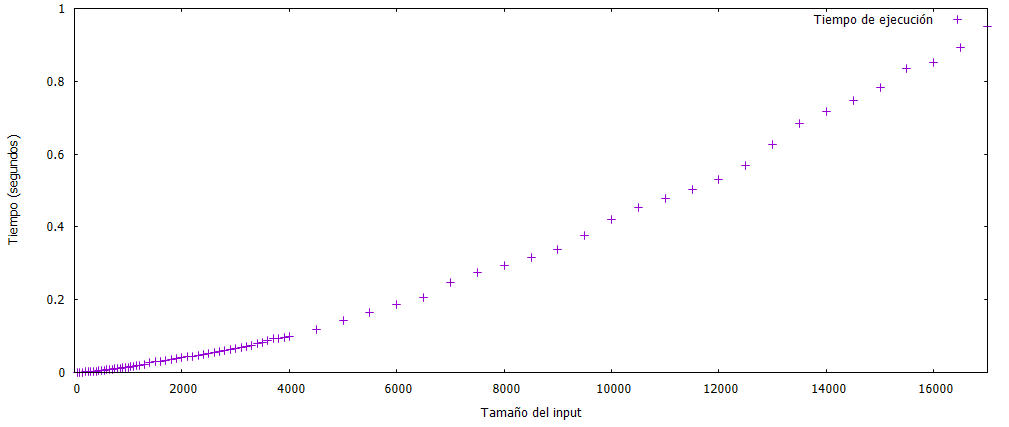
\includegraphics[width=1\textwidth]
   	 	{Imagenes/medianaTiempos.png}
		\caption{Tiempos variando el tama\~no del input}
	\end{figure}
	\\
	\newline
	\\Para el peor caso, se supuso que Java representa internamente al heap con un \'arbol binario, por lo que se dispuso a dise\~nar arreglos que fuercen a producir \textit{log n} intercambios cada vez que se realizaba una adici\'on al heap.
	\\Los arreglos que cumpl\'ian con esa propiedad eran aquellos que contenian n\'umeros en orden creciente en sus posiciones pares y n\'umeros en orden decresciente en sus posiciones impares (por ejemplo, (3, 89, 7, 62, 13, 50, 19, 43). De esta manera, por c\'omo se encuentra armado el algoritmo, siempre se agregaban elementos mayores que la ra\'iz al max heap y siempre se agregaban elementos menores que la ra\'iz al min heap (por lo que, te\'oricamente, se realizaban \textit{log n} intercambios en cada encolamiento).
	\\Sin embargo, al realizar los tests, si bien en un principio los tiempos eran mayores, al aumentar el tama\~no  del input, la funci\'on crec\'ia linealmente. Al desconocer c\'omo representa Java internamente a las colas de prioridad, no pudimos formar un caso que sea el peor.
	\\El tama\~no del input se fue aumentando en 100 desde el 0 al 1000 y en 500 del 1000 al 5000.
	\begin{figure}
  		\centering
   	 	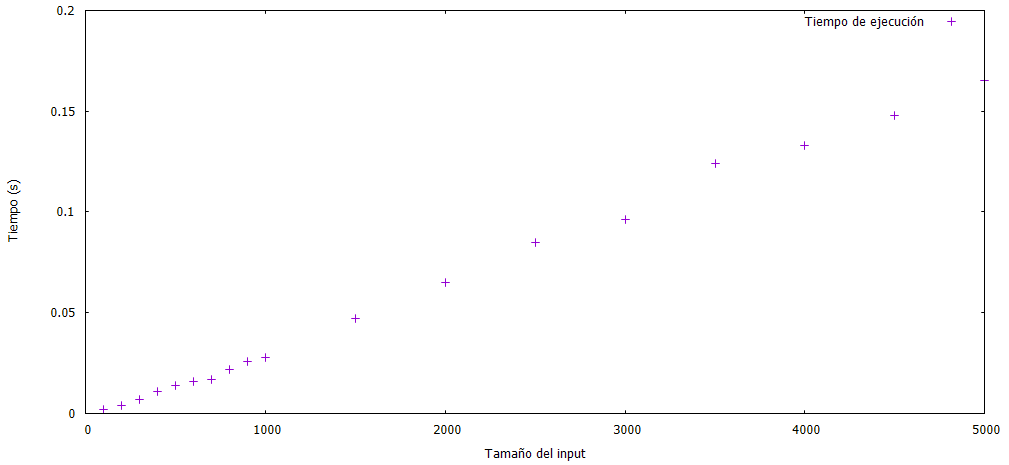
\includegraphics[width=1\textwidth]
   	 	{Imagenes/medianaPeorTiempos.png}
		\caption{Tiempos del peor caso variando el tama\~no del input}
	\end{figure}
\end{document}